%\acresetall
\definecolor{mGreen}{rgb}{0,0.6,0}
\definecolor{mGray}{rgb}{0.5,0.5,0.5}
\definecolor{mPurple}{rgb}{0.58,0,0.82}
\definecolor{backgroundColour}{rgb}{0.95,0.95,0.92}

\lstdefinestyle{CStyle}{
	%backgroundcolor=\color{backgroundColour},   
	commentstyle=\color{mGreen},
	keywordstyle=\color{blue},
	numberstyle=\tiny\color{mGray},
	stringstyle=\color{magenta},
	basicstyle=\footnotesize,
	breakatwhitespace=false,         
	breaklines=true,                 
	captionpos=b,                    
	keepspaces=true,                 
	%numbers=left,                    
	numbersep=5pt,                  
	showspaces=false,                
	showstringspaces=false,
	showtabs=false,                  
	tabsize=2,
	language=C
}
\chapter{Design and Implementation of Ferify}\label{ch:chapter3}

In this chapter, we discuss the design and the implementation choices that we made for this research, including the threat model and assumptions made.

\section{Overview}\label{sec:overview}

\par In this research, we extended the Xen hypervisor by leveraging its \ac{VMI} capabilities to create a system, which we called \codeft{ferify}. \codeft{Ferify} protects critical files on a \ac{VM}'s mounted filesystem by intercepting and monitoring \emph{all} systems calls that may operate on these files. It maintains its own file \acp{ACL} and allows a system call to read or write a file \emph{if, and only if,} the \ac{ACL} permits the action explicitly for the \ac{UID} and \ac{GID} combination of the calling process. We call this \ac{ACL} the \ac{SACL} to differentiate it from other \acp{ACL} configured on guest \acp{VM}. It is important to note that the content of the \ac{SACL} cannot be read nor modified by \emph{any} process, including kernel processes from guest \acp{VM}. The aforementioned permissions can be different compared to those on the guest \ac{VM}, allowing for the enforcement of different file access policies than the ones enforced by the guest \ac{VM}, even while under \ac{VM}-compromised attacks. The \ac{ACL} policies enforced by the guest \ac{OS} remain active, meaning that if for some reason the \ac{SACL} entry allows file access, but the guest \ac{OS} \ac{ACL} does not, the file will not be accessed.

\par First, before presenting the design and implementation details, we briefly discuss why our solution is secure: we choose to monitor which files were being accessed by trapping the system calls that are being invoked. 

\par As mentioned in \cite{linuxkernel}, a User Mode process cannot directly access the hardware; each file operation must be performed in Kernel Mode as the \ac{OS} will not allow direct access to hardware. If a process needs file access, it must perform a system call, asking the \ac{OS} in this way for the desired operation. The \ac{OS} checks if the request is valid and, if it is, accesses the file on behalf of the process and returns the result of the operations to the process, as shown in Figure~\ref{fig:syscall}. This requirement of making a system call for \emph{all} file operations provides a place in the \ac{OS} executable code, which, if we monitor, we can extract the information of all files being accessed. So, we cannot miss \emph{any file} that \emph{any process} tries to open.

\begin{figure}[ht]
	\centering
	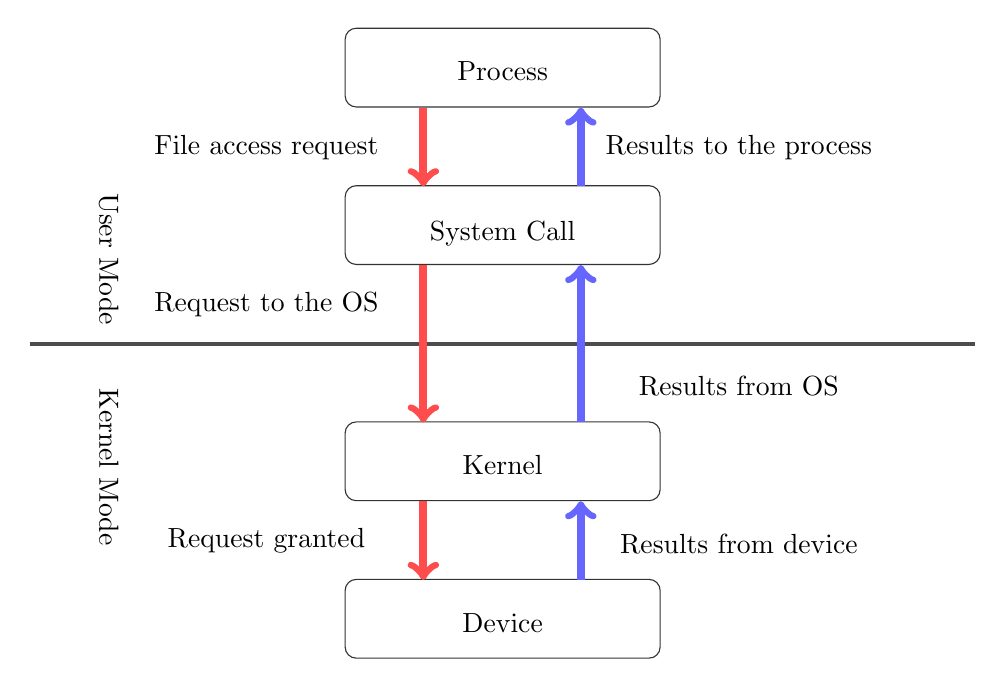
\begin{tikzpicture}[
rednode/.style={circle, draw=red!60, fill=red!30, very thick, minimum size=5mm, text width=2cm, text centered},
bluenode/.style={rectangle, draw=black!60, fill=blue!20, very thick, minimum size=5mm, text width=2cm, text centered},]



\node (rect) [anchor= south west, fill=white, rectangle, draw=black!80, rounded corners, minimum width=40mm, minimum height=10mm, label={[yshift=-0.8cm]Process}] at (2, 0) {}; 

\node (rect) [anchor= south west, rectangle, rounded corners, minimum width=20mm, minimum height=10mm, label={[yshift=-0.9cm]File access request}] at (0, -0.9) {}; 

\node (rect) [anchor= south west, rectangle, rounded corners, minimum width=20mm, minimum height=10mm, label={[yshift=-0.9cm]Results to the process}] at (6, -0.9) {}; 

\node (rect) [anchor= south west, fill=white, rectangle, draw=black!80, rounded corners, minimum width=40mm, minimum height=10mm, label={[yshift=-0.9cm]System Call}] at (2, -2) {}; 

\node (rect) [anchor= south west, rectangle, rounded corners, minimum width=20mm, minimum height=10mm, label={[yshift=-0.9cm]Request to the \ac{OS}}] at (0, -2.9) {}; 

\node (rect) [anchor= south west, rectangle, rounded corners, minimum width=20mm, minimum height=10mm, label={[yshift=-0.9cm]\rotatebox{270}{User Mode}}] at (-2, -3) {}; 

\draw[anchor= south west, draw=black!70, line width=0.5mm,-] (-2, -3) -- (10, -3);

\node (rect) [anchor= south west, rectangle, rounded corners, minimum width=20mm, minimum height=10mm, label={[yshift=-0.7cm]\rotatebox{270}{Kernel Mode}}] at (-2, -6) {}; 

\node (rect) [anchor= south west, fill=white, rectangle, draw=black!80, rounded corners, minimum width=40mm, minimum height=10mm, label={[yshift=-0.8cm]Kernel}] at (2, -5) {}; 

\node (rect) [anchor= south west, rectangle, rounded corners, minimum width=20mm, minimum height=10mm, label={[yshift=-0.9cm]Results from \ac{OS}}] at (6, -3.9) {}; 

\node (rect) [anchor= south west, rectangle, rounded corners, minimum width=20mm, minimum height=10mm, label={[yshift=-0.9cm]Request granted}] at (0, -5.9) {}; 

\node (rect) [anchor= south west, rectangle, rounded corners, minimum width=20mm, minimum height=10mm, label={[yshift=-0.9cm]Results from device}] at (6, -5.9) {}; 

\node (rect) [anchor= south west, fill=white, rectangle, draw=black!80, rounded corners, minimum width=40mm, minimum height=10mm, label={[yshift=-0.8cm]Device}] at (2, -7) {}; 

\draw[anchor= south west, draw=red!70, line width=1mm,->] (3, 0) -- (3, -1);
\draw[anchor= south west, draw=red!70, line width=1mm,->] (3, -2) -- (3, -4);
\draw[anchor= south west, draw=red!70, line width=1mm,->] (3, -5) -- (3, -6);

\draw[anchor= south west, draw=blue!60, line width=1mm,<-] (5, 0) -- (5, -1);
\draw[anchor= south west, draw=blue!60, line width=1mm,<-] (5, -2) -- (5, -4);
\draw[anchor= south west, draw=blue!60, line width=1mm,<-] (5, -5) -- (5, -6);


%\draw[anchor= south west, draw=red!70, line width=1mm,->] (4.5, 2) -- (7.2, 2);
%\draw[anchor= south west, draw=red!70, line width=1mm,->] (9.2, 2) -- (9.6, 2);
%\draw[anchor= south west, draw=red!70, line width=1mm,->] (11.6, 2) -- (12.2, 2);

%\draw[anchor= south west, draw=blue!60, line width=1mm,->] (12.2, 1) -- (1, 1) -- (1, 3.5);
%\draw[anchor= south west, draw=blue!60, line width=1mm,->] (1, 4.5) -- (1, 5);



\end{tikzpicture}
	\caption{System call information flow.}
	\label{fig:syscall}
\end{figure}

\par Table 12.1 in \cite{linuxkernel} shows the list of system calls relevant to filesystems. According to that table, the system calls of importance to us are \codeft{open()}, \codeft{rename()}, \codeft{link()}, \codeft{symlink()}, \codeft{unlink()}, and \codeft{truncate()}. Some of these system calls have evolved over time to provide better security and to eliminate problems. Such an evolved system call is \codeft{openat()}. Going through the available system call list in \codeft{/usr/include/asm/unistd\_64.h}, we assess that the system calls mentioned in Table~\ref{tbl:syscalls},\footnote{The column ``Number'' in Table \ref{tbl:syscalls} represents the system call number as it is passed to the kernel.} provide \emph{full coverage} of the possible ways a file can be accessed when being on a mounted device. 

\par As explained in \cite{perla2010guide}, it is possible for an attacker to modify the credentials of a process after acquiring root privileges. This exploit is a significant security issue for \codeft{ferify}, since it collects the \ac{UID} and \ac{GID} of the running process from the \ac{VM}'s kernel memory. To avoid the success of such an exploit, \codeft{ferify} monitors the credentials of \emph{all} running processes inside the guest \ac{VM}, and monitors the creation of new processes to record their credentials as well. Then, according to preset rules, \codeft{ferify} decides whether a change in the credentials of a process is allowed or not and acts accordingly. This way, we can secure the validity of the information collected from the guest \ac{VM}.


\begin{table}[ht]
	\centering
	\caption{Trapped system calls related to file operations}
	\label{tbl:syscalls}
	\begin{tabular}{cc|cc}
		\toprule
		\textbf{System call} & \textbf{Number} & \textbf{System call} & \textbf{Number} \\
		\hline
		\codeftfs{open()} 					& \codeftfs{2} 		& 
		\codeftfs{openat()} 				& \codeftfs{257} 	\\ 
		\codeftfs{name\_to\_handle\_at()}	& \codeftfs{303} 	&
		\codeftfs{open\_by\_handle\_at()} 	& \codeftfs{304} 	\\
		\codeftfs{rename()}					& \codeftfs{82} 	& 
		\codeftfs{renameat()}				& \codeftfs{264} 	\\  
		\codeftfs{renameat2()} 				& \codeftfs{316} 	& 
		\codeftfs{truncate()} 				& \codeftfs{76} 	\\
		\codeftfs{link()} 					& \codeftfs{86} 	&
		\codeftfs{linkat()} 				& \codeftfs{265}	\\
		\codeftfs{symlink()} 				& \codeftfs{88} 	&
		\codeftfs{symlinkat()} 				& \codeftfs{266} 	\\
		\codeftfs{unlink()} 				& \codeftfs{87} 	&
		\codeftfs{unlinkat()} 				& \codeftfs{263} 	\\
		\codeftfs{execve()} 				& \codeftfs{59} 	&
		\codeftfs{execveat()} 				& \codeftfs{322} 	\\
		
		\bottomrule
	\end{tabular}	
\end{table}

\par LibVMI, and therefore DRAKVUF, needs for the guest \ac{VM} to have reached a state, after launching, in which it is able to start monitoring the guest \ac{VM}. After we launch a VM there might be a small time window in which the guest \ac{VM} is running without the protection of our system. Until we find a way to determine the exact amount of time in which LibVMI can be initialized to protect the guest \ac{VM}, we will consider attacks that modify the running system during boot time outside the scope of this research. To prevent the system from being attacked during that small time frame, we do not connect the \ac{VM} to the network until after this initialization process is completed. 

\section{Threat Model}\label{sec:threat}

Computer security has been evolving because the attackers' methods evolve, too. Modern \acp{OS} and applications are so complex that they inevitably introduce many bugs in their code. Some of these bugs are benign, but some are serious enough to allow security breaches like remote access to a system, administrator/root access, or arbitrary code execution.

\par For this research, we have adopted a \emph{moderate} threat model where we assume that the guest \ac{VM} is insecure. We assume that physical access to the hosting machine is restricted and the attacker cannot use physical media like USB sticks or CD-ROMs to compromise the host system. The protected files are only remotely accessible and protected  by  a  public-key  authentication  and  encryption scheme (i.e., \emph{SSH}). The  private  keys  of  authorized  users  are  secure, while the attacker may have obtained root privileges on the \ac{VM} through a successful attack. The assumption that the target \ac{VM} would only be accessible remotely reflects many applications and systems working over a network connection as well as cloud solutions. A significant  concern  in  computer security is that of replay attacks. Even if a legitimate user connects using \emph{SSH}, there are attacks that can monitor  network  traffic  on  the  host  and  steal  sensitive data after they are decrypted. We consider these types of attacks and how to mitigate them outside the scope of this research, as the \emph{SSH} protocol is widely used and evolving. Finally, the files we want to protect are on a mounted disk.

\par Moreover, we assume that the \ac{OS} installed on the guest \ac{VM} is not trusted. This essentially means that the adversaries could gain root privileges, allowing them to modify system executables this way, as well as load kernel modules during runtime. This allows for kernel memory modification.

\par We consider the hypervisor, along with its Dom0, to be secure and trusted; hypervisor vectored attacks or how to protect the hypervisor is outside the scope of this research.

\section{Requirements}\label{sec:requirements}
The goal of this research is to provide a virtualization extension that will extend the granular-level file access control of the Linux \ac{OS}. The requirements we have defined for our system are:
\begin{itemize}
	\item \textbf{(R1)} The solution must be \emph{out-\ac{VM}} to avoid modification from the potential adversary. 
	\item \textbf{(R2)} The system must remain \emph{efficient and usable} by not introducing significant overhead on the runtime of the \ac{VM}, as well as by not enforcing many restrictions to the users. 
	\item \textbf{(R3)} \emph{All} relevant system calls must be monitored.
\end{itemize}


\section{Design}\label{sec:design}

\par We used a type-I hypervisor, as this type is more efficient and deployed more often as commercial solutions, instead of type-II, which is used mostly for testing and analysis. We chose the Xen hypervisor as it is open-source and is used widely, so the results of the research can be used in a variety of applications. By leveraging Xen's introspection methods, we created an \emph{Out-\ac{VM}} monitoring agent,\footnote{Out-\ac{VM} means that the agent runs on Dom0.} completely \emph{outside} the \ac{VM}, conforming this way with \textbf{(R1)}. Also, by ensuring that there is no code running on the guest \ac{OS}, we have increased the deployment speed, as there is no need to modify the guest \ac{VM} in any way. The required pre-deployment configuration for the guest \ac{VM} is kept to a minimum and does not involve any modification, only data collection for building the \acp{SACL}.

\par As a platform on which to base our solution, we chose DRAKVUF~\cite{lengyel2014drakvuf}. DRAKVUF provided us with a stealthy monitoring base, as it leverages alternate \ac{EPT}s with different permissions, thus preventing any detection from applications inside a \ac{VM}. As explained later in this chapter, we had to restrict some of the usability of the system, although not during normal execution, to achieve the file \emph{confidentiality}, \emph{integrity}, and \emph{availability} we wanted. Therefore, we assumed that \textbf{(R2)} is achieved in the part of restrictions, although a few restrictions apply, mostly concerning the root user. Overhead and usability of the system is discussed in Chapter~\ref{ch:chapter4}.

\par Generally, we wanted to protect any type of data, regardless of the content. We employed the stealthy property of DRAKVUF to make the process of file protection completely transparent to the guest \ac{OS}, retaining a zero-footprint monitor on the guest. By having access to selected kernel structures, DRAKVUF also helps bridge the semantic gap between the hypervisor and the \ac{VM} with the use of a Rekall profile~\cite{rekall}. Furthermore, we wanted to employ a per-user \ac{ACL}, to be enforced on specific files or whole folders; these are not always essential to the \ac{OS}, but are essential to the user. We improved \emph{confidentiality} by denying read access, \emph{integrity} by denying write, and \emph{availability} by protecting deletion or moving of files. Since our threat model assumes that the system is compromised, this mechanism must also extend to the root user. To achieve that, we intercept \emph{all} relevant system calls from \emph{all} users and verify the validity of the request. 

\par Monitoring the execution of the system calls in Table~\ref{tbl:syscalls} and validating the request made to the guest \ac{OS} kernel is sufficient for ensuring the guest \ac{VM} file confidentiality, integrity, and availability as we want to enforce it, thus conforming to \textbf{(R3)}.


\section{Implementation}\label{sec:implementation}

\par In the following discussion, we expand on how we implemented the mechanism to provide the file access security of our system.

\subsection{Architecture}\label{sub:arch}

\par We developed \codeft{ferify} as a plugin for DRAKVUF. As such, it is a C++ class that extends the class \codeft{plugin}, as per requirements of DRAKVUF. It is located in the directory \codeft{src/plugins/ferify/} and consists of two files, \codeft{ferify.h} and \codeft{ferify.cpp}, as shown in Figure~\ref{fig:dir_tree}. 

\begin{figure}[ht]
	\centering
	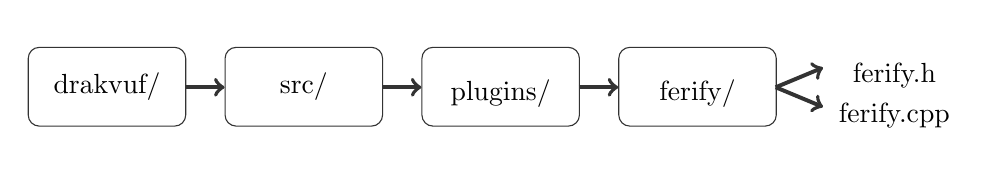
\begin{tikzpicture}[
rednode/.style={circle, draw=red!60, fill=red!30, very thick, minimum size=5mm, text width=2cm, text centered},
bluenode/.style={rectangle, draw=black!60, fill=blue!20, very thick, minimum size=5mm, text width=2cm, text centered},]



\node (rect) [anchor= south west, fill=white, rectangle, draw=black!80, rounded corners, minimum width=20mm, minimum height=10mm, label={[yshift=-0.8cm]drakvuf/}] at (0, 0) {}; 

\node (rect) [anchor= south west, fill=white, rectangle, draw=black!80, rounded corners, minimum width=20mm, minimum height=10mm, label={[yshift=-0.8cm]src/}] at (2.5, 0) {}; 

\node (rect) [anchor= south west, fill=white, rectangle, draw=black!80, rounded corners, minimum width=20mm, minimum height=10mm, label={[yshift=-0.9cm]plugins/}] at (5, 0) {}; 

\node (rect) [anchor= south west, fill=white, rectangle, draw=black!80, rounded corners, minimum width=20mm, minimum height=10mm, label={[yshift=-0.9cm]ferify/}] at (7.5, 0) {}; 

\node (rect) [anchor= south west, rectangle, rounded corners, minimum width=20mm, minimum height=10mm, label={[yshift=-0.9cm]ferify.h}] at (10, 0.25) {}; 

\node (rect) [anchor= south west, rectangle, rounded corners, minimum width=20mm, minimum height=10mm, label={[yshift=-0.9cm]ferify.cpp}] at (10, -0.25) {}; 

\draw[anchor= south west, draw=black!80, line width=0.5mm,->] (2, 0.5) -- (2.5, 0.5);
\draw[anchor= south west, draw=black!80, line width=0.5mm,->] (4.5, 0.5) -- (5, 0.5);
\draw[anchor= south west, draw=black!80, line width=0.5mm,->] (7, 0.5) -- (7.5, 0.5);
\draw[anchor= south west, draw=black!80, line width=0.5mm,->] (9.5, 0.5) -- (10.1, 0.75);
\draw[anchor= south west, draw=black!80, line width=0.5mm,->] (9.5, 0.5) -- (10.1, 0.25);


\end{tikzpicture}
	\caption{\codeft{ferify} directory tree.}
	\label{fig:dir_tree}
\end{figure}

\subsection{Shadow Access Control List}\label{sub:sacl}
During the initialization of our DRAKVUF plugin, we read the \ac{SACL}s we had created for the \ac{VM} to be protected. The \acp{SACL} are implemented in the form of hash tables in order to improve search speed. The key of the hash table is the full pathname of the file and the value is a structure, depicted in Table~\ref{tbl:sacl_layout}, used to store the rest of each \ac{SACL} entry's information.

\begin{table}[ht]
	\centering
	\begin{tabular}{cc}
		%\hline
		\textbf{Variable Name} & \textbf{Variable type} \\
		\hline
		\codeft{pathname} & 
		\codeft{char *} \\
		%\hline
		\codeft{mode} & 
		\codeft{unsigned int} \\
		%\hline
		\codeft{u} & 
		\codeft{uid\_t} \\
		%\hline
		\codeft{g} & 
		\codeft{gid\_t} \\
		\hline
	\end{tabular}
	\caption{\codeft{struct protected\_files} memory layout.}
	\label{tbl:sacl_layout}
\end{table}

\par The memory structure shown in Table~\ref{tbl:sacl_layout} is used for both protected folders and protected files, as they are handled the same. Moreover, we create two; one for the root user and one for the rest. Searching in the \acp{SACL} is performed with the pathname of the file being accessed as the hash-table key. The return value is a pointer to the structure of Table~\ref{tbl:sacl_layout}. 

\par In the \ac{SACL} file, permissions are set according to the Linux permission bits schema. This means that the last three digits of the \textit{mode} field, when encoded in octal form, define the permissions we want to enforce. The first digit defines the owner permissions, the second the group permissions, and the third the other user permissions. The number itself is the sum of the permissions: 4 for read, 2 for write, and 1 for execute. As an example, if we encounter or set permissions 744, it means that the owner can read, write, and execute the file; everyone else can only read the file.

\par The \ac{SACL}'s format was kept as simple as possible so that editing and reviewing it is easy. Additionally, by keeping the format of the Linux \ac{ACL}, we provide the system administrator with a familiar permissions schema so it is easier to understand and manage. Figure~\ref{fig:sacl} shows an example, which we analyze later.

\begin{figure}[ht]
	\centering
	\begin{tabular}{lccc}
Pathname&Permissions&User&Group\\
\hline
\codeft{/home/user/Documents/readme.txt} & 
	\codeft{100644} & \codeft{1000} & \codeft{1000}\\
\codeft{/home/user/Desktop/credit.pdf}	 & 
	\codeft{100400} & \codeft{1000} & \codeft{1000}\\
\codeft{/home/user/Documents}			 & 
	\codeft{140220} & \codeft{0}    & \codeft{0}\\
	\hline
	\end{tabular}
	\caption{\ac{SACL} sample.}
	\label{fig:sacl}
\end{figure}

\par The system keeps two \acp{SACL}: one for all non-root users and one for root, since this account is of greater significance. Furthermore, two different checks are performed. First, \codeft{ferify} checks for a protected folder, or a parent, as this is a more generic case. If no entry is found, it then checks for specific files that match those in the list. 

\par We chose to create two separate \acp{SACL} to improve the permissions policy of our solution. By making this separation we allow for the creation of separate permissions for normal users and the root user. It makes managing of different permissions easier. 
%the program to automatically eliminate entries in the \ac{SACL} that need not be checked against. If a program or service runs as root, we do not need to check the entries that apply to the rest of the users and vice versa. Additionally, since the root user account will always run on a system, because the \ac{OS} runs under this account, root will constantly open files relevant to the running of the \ac{OS}. Therefore, we assess that adding more entries to match against in the \ac{SACL} will introduce a performance overhead we can avoid with the separation we implemented. 
Besides this simple refinement of the \ac{SACL} entries, the level of protection applied to the files is the same for any user.

\par As we see in Figure~\ref{fig:root_sacl}, the \ac{SACL} for protecting files from the root user is simpler. Since it is targeted for this specific user, we do not need the entries for the owner or group. Furthermore, the permission bits for group and others are ignored when parsed, since they are meaningless.

\begin{figure}[ht]
\centering
\begin{tabular}{lc}
	Pathname&Permissions	\\
	\hline
%	\footnotesize{\fontfamily{qcr}\selectfont 
	\codeft{/etc/shadow}  &  \codeft{100400}\\
	\codeft{/etc/pam.d/su} & \codeft{100000}\\
	\hline
\end{tabular}
	\caption{root user \ac{SACL} sample.}
	\label{fig:root_sacl}
\end{figure}


\par Before moving on, we must emphasize that the system does not alter basic properties of the files that are being protected, nor does it change the owner or the group, since this requires intervention in the \ac{VM}. Although in the \ac{SACL} we can define a different owner, the generic effect is denial of access. This means that we cannot change who can access a file; rather, we can change who cannot. This system acts as a supplementary and more refined access control mechanism to make more strict file access policies. Therefore, if we change the owner of a file in the \ac{SACL}, we essentially prohibit access to that file by the owner. Similarly, we do specify a new one, as the final call for file access comes from the unmodified guest \ac{OS}.



\subsection{System Call Interception and Admission Control}\label{sub:syscalls}


\par All applications running in user space need to ask the kernel to access a file. Applications do not have knowledge of the low-level \ac{OS} and device details to access the files they need, so they request the kernel to do that work for them. The kernel accesses the requested file using the device drivers and, when the operation is completed, returns to the application a handle to that file.\footnote{The handle to the file is called the file descriptor.} This happens for many operations restricted to the kernel for security reasons. Also, it provides an abstraction to the applications, which are written without the need for knowledge of device specifics, and works on variations of the underlying hardware running the same \ac{OS}. 

\par For applications to be compatible with \ac{OS} version upgrades and portable between different systems, a specific standard calling convention of these kernel functions is needed. This calling convention is a system call. System calls are specific entry points to the kernel which, when provided specific arguments, perform an operation on behalf of the application. Many system calls exist, each performing a different operation. We focus on those that are relevant to accessing files, whether to read or modify. These are depicted in Table~\ref{tbl:syscalls}.

\par To gain the insight needed on what files are being accessed, we need to know whenever this event happens. We will use DRAKVUF to create a trap on all the aforementioned system calls; this gives us the opportunity to stop the \ac{VM} execution when these system calls are made. At this point, we will access the registers related with each system call to retrieve the information we need to perform the validation of the requested call. Figure~\ref{fig:overview} gives an overview of the flow of information during a trapped system call. 

\par The arguments for the system calls for the 64-bit Linux \ac{OS} we used as our test platform are passed to the kernel through the registers in the order of \codeft{rdi}, \codeft{rsi}, \codeft{rdx}, \codeft{r10}, \codeft{r8}, and \codeft{r9}, while the system call number is passed in \codeft{rax}. Additionally, \codeft{rcx} holds the return address for execution after the system call has been completed. Table~\ref{tbl:prototypes} shows which arguments need to be passed to each system call on each register for it to perform the requested operation, as found online~\cite{syscalls}.

\begin{table}[ht]
\centering
\footnotesize
\caption{Arguments of file related trapped system calls}
\label{tbl:prototypes}			
\begin{tabular}{ccccccc}
	\toprule
	\textbf{Syscall Name} & \textbf{rax} & \textbf{rdi} & \textbf{rsi} & \textbf{rdx} & \textbf{r10} & \textbf{r8}\\
	\toprule
	%%%
	\codeftsm{open}					& 
	\codeftsm{2} 					&		
	\codeftsm{const char}			&	
	\codeftsm{int}					&
	\codeftsm{int}					&&\\
	%%%
	&&	
	\codeftsm{*pathname}			&
	\codeftsm{flags}				&
	\codeftsm{mode}					&&\\
	%%%
	\hline
	%%%
	\codeftsm{openat}				& 
	\codeftsm{257} 					&	
	\codeftsm{int}					&
	\codeftsm{const char}			&
	\codeftsm{int}					&
	\codeftsm{int}					&\\
	%%%
									&&		
	\codeftsm{dirfd}				&
	\codeftsm{*pathname}			&
	\codeftsm{flags}				&
	\codeftsm{mode}					&\\
	%%%
	\hline
	%%%	
	\codeftsm{name\_to\_handle\_at} &
	\codeftsm{303}  				&	
	\codeftsm{int}					&	
	\codeftsm{const char}			&	
	\codeftsm{struct}				&	
	\codeftsm{int}					&	
	\codeftsm{int}	 				\\
	%%%
	&&
	\codeftsm{dirfd}				&	
	\codeftsm{*pathname}			& 
	\codeftsm{file\_handle} 		&
	\codeftsm{mount\_id}			&
	\codeftsm{flags}				\\
	%%%
	&&&&
	\codeftsm{*handle}				&&\\
	%%%
	\hline
	%%%	
	\codeftsm{open\_by\_handle\_at} & 
	\codeftsm{304}  				&	
	\codeftsm{int}					&	
	\codeftsm{struct}				&	
	\codeftsm{int}					&&\\
	%%%
	&&	
	\codeftsm{mountfd}				&	
	\codeftsm{file\_handle}			&
 	\codeftsm{flags}				&&\\
 	%%%
	&&&	
	\codeftsm{*handle}				&&&\\
	%%%
	\hline
	%%%	
	\codeftsm{rename} 				& 
	\codeftsm{82}  					&	
	\codeftsm{const char}			&	
	\codeftsm{const char}			&&&\\
	%%%
	&&	
	\codeftsm{*oldpath}				&	
	\codeftsm{*newpath}				&&&\\
	%%%
	\hline
	%%%
	\codeftsm{renameat} 			& 
	\codeftsm{264}  				&	
	\codeftsm{int} 					&	
	\codeftsm{const char} 			&	
	\codeftsm{int} 					&	
	\codeftsm{const char} 			&\\
	%%%
	&&	
	\codeftsm{olddirfd}				&	
	\codeftsm{*oldpath}				&	
	\codeftsm{newdirfd}				&	
	\codeftsm{*newpath}				&\\ 
	%%%
	\hline
	%%%
	\codeftsm{renameat2} 			& 
	\codeftsm{316}  				&
	\codeftsm{int}					&	
	\codeftsm{const char} 			&	
	\codeftsm{int} 					&		
	\codeftsm{const char} 			&	
	\codeftsm{int}					\\
	%%%
	&&	
	\codeftsm{olddirfd}				&	
	\codeftsm{*oldpath}				&	
	\codeftsm{newdirfd}				&	
	\codeftsm{*newpath}				&
	\codeftsm{flags}				\\
	%%%
	\hline
	%%%
	\codeftsm{link} 				& 
	\codeftsm{86}  					&	
	\codeftsm{const char}			&	
	\codeftsm{const char}			&&&\\
	%%%
	&&	
	\codeftsm{*oldpath}				&	
	\codeftsm{*newpath}				&&&\\
	%%%
	\hline
	%%%
	\codeftsm{linkat} 				& 
	\codeftsm{265}  				&	
	\codeftsm{int}					&	
	\codeftsm{const char} 			&	
	\codeftsm{int} 					&		
	\codeftsm{const char} 			&	
	\codeftsm{int}					\\
	%%%
	&&	
	\codeftsm{olddirfd}				&	
	\codeftsm{*oldpath}				&	
	\codeftsm{newdirfd}				&	
	\codeftsm{*newpath}				&
	\codeftsm{flags}				\\		
	%%%
	\hline
	%%%
	\codeftsm{symlink} 				& 
	\codeftsm{88}  					&	
	\codeftsm{const char}			&	
	\codeftsm{const char}			&&&\\
	%%%
	&&	
	\codeftsm{*oldpath}				&	
	\codeftsm{*newpath}				&&&\\
	%%%
	\hline
	%%%
	\codeftsm{symlinkat} 			& 
	\codeftsm{266}  				&	
	\codeftsm{const char}			&
	\codeftsm{int}					&
	\codeftsm{const char}			&&\\
	%%%
	&&	
	\codeftsm{*oldpath}				&
	\codeftsm{newdirfd}				&	
	\codeftsm{*newpath}				&&\\
	%%%
	\hline
	%%%
	\codeftsm{unlink} 				& 
	\codeftsm{87}  					&	
	\codeftsm{const char}			&&&&\\
	%%%
	&&	
	\codeftsm{*pathname}			&&&&\\ 
	%%%
	\hline
	%%%
	\codeftsm{unlinkat} 			& 
	\codeftsm{263}  				&	
	\codeftsm{int}					&	
	\codeftsm{const char}			&	
	\codeftsm{int}					&&\\
	%%%
	&&
	\codeftsm{dirfd}				&	
	\codeftsm{*pathname}			&
	\codeftsm{flag}					&&\\
	%%%
	\hline
	%%%
	\codeftsm{truncate} 			& 
	\codeftsm{76}  					&	
	\codeftsm{const char}			&	
	\codeftsm{off\_t}				&	
	\codeftsm{int}					&&\\
	%%%
	&&	
	\codeftsm{*pathname}			&	
	\codeftsm{length}				&
	\codeftsm{flag}					&&\\
	%%%
	\hline
	%%%
	\codeftsm{execve} 				& 
	\codeftsm{59}  					&	
	\codeftsm{const char}			&	
	\codeftsm{char *const}			&	
	\codeftsm{char *const}			&&\\
	%%
	&&	
	\codeftsm{*filename}			&	
	\codeftsm{argv[]}				&
	\codeftsm{envp[]}				&&\\
	%%%
	\hline
	%%%
	\codeftsm{execveat} 			& 
	\codeftsm{322}  				&	
	\codeftsm{int}					&	
	\codeftsm{const char}			&	
	\codeftsm{char *const}			&
	\codeftsm{char *const} 			&
	\codeftsm{int}					\\
	%%%
	&&	
	\codeftsm{dirfd}				&	
	\codeftsm{*pathname}			&
	\codeftsm{argv[]}				&
	\codeftsm{envp[]}				&
	\codeftsm{flags}				\\

	\bottomrule
\end{tabular}
\end{table}



\begin{figure}[ht]
	\centering
	\begin{tikzpicture}[
rednode/.style={circle, draw=red!60, fill=red!30, very thick, minimum size=5mm, text width=2cm, text centered},
bluenode/.style={rectangle, draw=black!60, fill=blue!20, very thick, minimum size=5mm, text width=2cm, text centered},]

  
   	\node[anchor= south west, copy shadow={draw=black!10, fill=black!40, opacity=0.5}, fill=white, rectangle, rounded corners, draw=black, minimum width=50mm, minimum height=80mm, label={[yshift=-1cm]north:Dom0}] at (0, 0) {};
   	
	\node[dashed, anchor= south west, fill=white, rectangle, draw=black!80, rounded corners, minimum width=45mm, minimum height=10mm, label={[yshift=-0.8cm]\ac{SACL}}] at (0.25, 6) {}; 
	\node[anchor= south west, fill=white, rectangle, draw=black!80, rounded corners, minimum width=45mm, minimum height=10mm, label={[yshift=-0.9cm]DRAKVUF Plugin}] at (0.25, 4.5) {}; 
	\node (rect) [anchor= south west, fill=white, rectangle, draw=black!80, rounded corners, minimum width=45mm, minimum height=10mm, label={[yshift=-0.8cm]LibVMI}] at (0.25, 3) {}; 
	
%	\node[dashed, anchor= south west, fill=white, rectangle, draw=black!80, minimum width=20mm, minimum height=15mm, label={[yshift=-1.5cm]\begin{tabular}{c}
%		System \\ Map
%		\end{tabular}}] at (2.5, 1.5) {}; 
	
	
   	\node[anchor= south west, copy shadow={draw=black!10, fill=black!40, opacity=0.5}, fill=white, rectangle, rounded corners, draw=black, minimum width=50mm, minimum height=70mm, label={[yshift=-0.7cm]north:User VM (DomU)}] at (7, 0) {};
	
	\node[anchor= south west, fill=white, rectangle, draw=black!80, rounded corners, minimum width=45mm, minimum height=10mm, label={[yshift=-0.8cm]User-level Application}] at (7.25, 4.5) {}; 
	\node[anchor= south west, fill=white, rectangle, draw=black!80, rounded corners, minimum width=45mm, minimum height=10mm, label={[yshift=-0.8cm]System Call}] at (7.25, 3) {}; 
	
	

%	\node[dashed, anchor= south west, fill=white, rectangle, draw=black!80, minimum width=20mm, minimum height=20mm, label={[yshift=-1.7cm]\begin{tabular}{c}
%		Page \\ Directory
%		\end{tabular}}] at (7.2, 1.5) {}; 
%
%	\node[dashed, anchor= south west, fill=white, rectangle, draw=black!80, minimum width=20mm, minimum height=20mm, label={[yshift=-1.7cm]\begin{tabular}{c}
%	Page \\ Table
%	\end{tabular}}] at (9.6, 1.5) {}; 
%
%	\node[dashed, anchor= south west, fill=white, rectangle, draw=black!80, minimum width=20mm, minimum height=20mm, label={[yshift=-1.7cm]\begin{tabular}{c}
%	Kernel \\ Data
%	\end{tabular}}] at (12.2, 0.5) {}; 
%
	\draw[anchor= south west, draw=red!70, line width=1mm,->] (8, 4.5) -- (8, 4);
	\draw[anchor= south west, draw=red!70, line width=1mm,->] (8, 3) -- (8, 2.5) -- (4, 2.5) -- (4, 3);
	\draw[anchor= south west, draw=red!70, line width=1mm,->] (4, 4) -- (4, 4.5);
	\draw[anchor= south west, draw=red!70, line width=1mm,->] (4, 5.5) -- (4, 6);
			
	\draw[anchor= south west, draw=blue!70, line width=1mm,<-] (11, 4.5) -- (11, 4);
	\draw[anchor= south west, draw=blue!70, line width=1mm,<-] (11, 3) -- (11, 1.5) -- (1, 1.5) -- (1, 3);
	\draw[anchor= south west, draw=blue!70, line width=1mm,<-] (1, 4) -- (1, 4.5);
	\draw[anchor= south west, draw=blue!70, line width=1mm,<-] (1, 5.5) -- (1, 6);



\end{tikzpicture}
	\caption{Information flow during a trapped system call execution.}
	\label{fig:overview}
\end{figure}


\subsection{System Call Hooking}\label{sub:hooking}

\par To achieve the aforementioned system call intercept, we need to place traps to the system calls of interest. These get implemented by DRAKVUF; LibVMI reads the Rekall profile of the guest \ac{VM} to get the base address of the kernel symbol table. DRAKVUF then starts from that base address and searches for the system call table. This table includes the function pointers for all supported system calls. Going through that table makes the detection and trapping of system calls possible. This is achieved by reading the address of the system call from the system call table, going to that address, and placing the \codeft{INT3 (0xCC)} byte at the beginning of the system call function. This does not alter the system call table; the system call table is stored information, while the injected byte is written in the actual code section. This byte is executed by the \ac{CPU} as a debugging interrupt or a breakpoint. This in turn triggers a VM-exit, which is caught by DRAKVUF and handled by our callback function. DRAKVUF implements multiple \ac{EPT}s with different permissions for the same page; this allows placing the trap in the system calls code. When the particular page is accessed for reading, an exception is raised, which is caught by the hypervisor. While the \ac{VM} is paused the hypervisor switches the page with the correct one and resumes the \ac{VM}. When the \ac{OS} tries to execute that part of code the opposite switch happens. The original function's code is accessed, without revealing the injected breakpoint. This process is transparent to the \ac{VM} because the contents of the pages are exactly the same, with the exception of the breakpoint, and all this happens when the \ac{VM} is paused. 

\par Table~\ref{tbl:prototypes} shows that there are two generic cases we need to examine. One case is for the \codeft{open()}, \codeft{rename()}, \codeft{link()}, \codeft{symlink()}, \codeft{unlink()}, and \codeft{truncate()} system calls, where we have to find the string pointed by the pointer in the \codeft{rdi} register, and in the \codeft{rsi} register in the case of \codeft{rename()}. 

\par The second case is for the \codeft{openat()}, \codeft{renameat()}, \codeft{renameat2()}, \codeft{linkat()}, \codeft{symlinkat()}, and \codeft{unlinkat()} system calls, where we have to retrieve the string of the file being accessed from different registers, according to Table~\ref{tbl:prototypes}. 




\subsection{The task\_struct Kernel Structure}\label{sub:struct}
\par A crucial part in the design of our solution is the Linux kernel \codeft{task\_struct}. It is a complex structure where the kernel stores extensive information concerning the running processes. Each running process is assigned one such structure by the kernel, so that the kernel can monitor the process and retrieve various information about it. A special macro, \codeft{current}, retrieves a pointer to the \codeft{task\_struct} of the currently running process.\footnote{The value is the return value of a function. Manipulating this value has no result, as each time it is called the correct value is always returned.} We then need to map this structure and find the address offsets of the information we need. We must make sure that the information we retrieve from the \codeft{task\_struct} is not corrupted, so we store the required information on the hypervisor, keeping track of all the processes. Additionally, to prevent a big attack surface on the kernel we decide to deny kernel module loading, as explained in detail in Subsection~\ref{sub:ring0}. We revisit the \codeft{task\_struct} in the next sections, as we mention what we need to access.

\par Although normally this process is not complex, in our case there were some challenges, such as the semantic gap already mentioned for all out-\ac{VM} solutions. The first is that we need to find the correct offsets inside the \codeft{task\_struct} for the entries we want, which depend on the kernel version. Furthermore, we need to make constant conversions between \ac{GMFN} and \ac{MFN}, as the memory values we retrieve correspond to the \ac{VM}s address space. Instead, we need to access the actual physical memory to read the information we require.


\subsection{Trap Handling}\label{sub:handling}

After a hooked system call gets executed, our callback function is called. We retrieve the file that is being accessed and, by getting the \codeft{current} process ID (Figure~\ref{fig:getfile}), we determine which process is making the system call. 

\begin{figure}[ht]
\fontfamily{qcr}\selectfont
\begin{lstlisting}[style=CStyle]
	currpid = vmi_dtb_to_pid(vmi, info->regs->cr3);
	switch (info->regs->rax){
		case S_OPEN:
		case S_RENAME:
		case S_UNLINK:
			addr=vmi_translate_uv2p(vmi,info->regs->rdi,currpid);
			filename=vmi_read_str_pa(vmi,addr);
			.
			.
			break;
		case S_OPENAT:
		case S_UNLINKAT:
		case S_RENAMEAT:
		case S_RENAMEAT2:
			addr=vmi_translate_uv2p(vmi,info->regs->rsi,currpid);
			filename=vmi_read_str_pa(vmi,addr);
			.
			.
			break;	
	}
\end{lstlisting}
	\caption{Getting the file being accessed.}
	\label{fig:getfile}
\end{figure}


\par When a system call is executed, the file being accessed is passed as a string pointer. After we retrieve the string, we check whether the file is given in the form of an absolute or relative path. If the path is absolute there is nothing more to do and the algorithm continues. If the path is relative, the retrieval procedure is more complicated because we need to recreate the \ac{PWD}. The Linux kernel does not store this information anywhere. On the contrary, in the \codeft{task\_struct}, the kernel only stores the parent directory in a different structure. Therefore, we need to loop through the parent folders so that by prepending the parent each time, we recreate the \ac{PWD} and the full pathname. To achieve this, we created a new function that recursively walks though the \codeft{task\_struct} to collect all the required information. 

\par The case for the \codeft{openat()}, \codeft{renameat()}, \codeft{renameat2()}, \codeft{linkat()}, \codeft{symlinkat()}, and \codeft{unlinkat()} system calls is different. Among the arguments, there is one called \codeft{dirfd}. This argument is not always used. When it is not, the algorithm is the same as described previously. When it is used, it is in the form of a directory descriptor. This means that the process has already successfully opened a directory and passed its descriptor as an argument, which represents the mount directory for the file. In this case we go through the \codeft{task\_struct} structure of the current running process and retrieve the directory that maps to the directory descriptor, so that we can recreate the pathname of the file.

\par After we have retrieved the pathname, we then check for the system call that triggered the VM-exit event. For this research, we will not handle the \codeft{name\_to\_handle\_at()} and \codeft{open\_by\_handle\_at()} system calls. At this point, we are unaware of any compiled program that uses this specific system call, but this does not hinder our proof of concept. Support for them can be added in the future. The rest of the system calls are handled as follows: 


\begin{itemize}
	\item \codeft{link()}, \codeft{linkat()}, \codeft{symlink()}, \codeft{symlinkat()}, \codeft{unlink()}, and \codeft{unlinkat()}
	\item \codeft{open()} and \codeft{openat()}
	\item \codeft{rename()}, \codeft{renameat()}, and \codeft{renameat2()}
\end{itemize}

\par In the first case, where the system calls are used for linking and file deletion, the procedure is straightforward. If there is an entry in the \ac{SACL}, we verify that the user or group accessing the file has sufficient permissions. If that is correct, the callback function returns control to the \ac{VM} to resume execution. If the permissions do not match, the pointer to the filename string is modified to \codeft{NULL} so that the system call, after the \ac{VM} resumes execution, fails (Figure~\ref{fig:unlink}). By hooking and preventing execution of these system calls, we prevent deletion and linking of the protected files, improving the \emph{availability} and \emph{confidentiality} assurances of the underlying \ac{OS}.

\par The search for a match in the \ac{SACL}s is performed in two steps for all cases: once to go through protected folders and once to go through individually protected files. Also, the root user is handled separately from the rest of the users because of the special elevated privileges that account is granted. 

\par In the case of \codeft{rename()}, \codeft{renameat()} and \codeft{renameat2()}, which are used for file moving, we perform the same check as per \codeft{unlink()} and \codeft{unlinkat()}, with the difference that if we do not find a match for the \codeft{oldname} of the system call, we additionally check for a match on the \codeft{newname}. As enforced by our \ac{SACL}, the first part ensures that if the user or group does not have read permissions, the file cannot be renamed or moved to an unprotected folder or filename, ensuring the \emph{confidentiality} of the information stored in the file. In the second case, we prevent the protected file from being overwritten by another file if the permissions are not correct. This way, we improve \emph{integrity} of the underlying \ac{OS} by preventing modification of the protected file. 

\begin{figure}[ht]
	\fontfamily{qcr}\selectfont
	\begin{lstlisting}[style=CStyle]
	
	case S_UNLINK:
	case S_UNLINKAT:
		switch(info->userid){
			case ROOT: // root user
				if(strcmp(check->pathname,filename)==0){
					check_permissions(check,info,vmi,ROOT);			
					.
					.
				break;
			default: // other users
				if (strcmp(check->pathname,filename)==0){
					if (check->u == info->userid){
						check_permissions(check,info,vmi,USER);}
					else if (check->g == info->groupid){
						check_permissions(check,info,vmi,GROUP);}
				else {
					check_permissions(check,info,vmi,OTHER);}
					.
					.
				break;
			}
	\end{lstlisting}
	\caption{unlink() and unlinkat() skeleton code flow.}
	\label{fig:unlink}
\end{figure}

\par Finally, in the case of \codeft{open()} and \codeft{openat()} we only must check for one filename in our \ac{SACL}s. If there is an entry, then the permission check algorithm is more complicated. This happens because we have to match the requested access mode with the permissions we want to enforce. So, we check for read permission when a \codeft{O\_RDONLY} access is requested, and for write permission on a \codeft{O\_WRONLY}. In the case of a \codeft{O\_RDWR} request, we initially check for both permissions. If that fails, we then check if the process user or group has read permissions. If that is the case, we alter the file access mode to read-only and allow execution. If all of them fail, we change the \codeft{rax} register contents to \codeft{NULL} and resume \ac{VM} execution; this results in a failed system call. This more complex permission check improves \emph{confidentiality} by not allowing read access to those who do not have the right, as well as \emph{integrity} and \emph{availability} by denying write access to those who cannot write to the file, as per the \ac{SACL}-enforced policy. Figure~\ref{fig:open} shows the code for the permission checks done in the case of the \codeft{open()} and \codeft{openat()} system calls.




\begin{figure}[ht!]
\fontfamily{qcr}\selectfont
\begin{lstlisting}[style=CStyle]
	switch(info->regs->rax){
		case S_OPEN:
		case S_OPENAT:
			if ( ((info->regs->rsi & 07) | O_RDONLY) == O_RDONLY){
				if ( !(check->mode & r) ) {
					vmi_set_vcpureg (vmi, 0, RDI, info->vcpu);
					return 1; }
			} else if ( ((info->regs->rsi & 07) | O_WRONLY) == O_WRONLY) {
				if ( !(check->mode & w) ) {
					vmi_set_vcpureg (vmi, 0, RDI, info->vcpu);
					return 1; }
			} else if ( ((info->regs->rsi & 07) | O_RDWR) == O_RDWR) {
				if ( !(check->mode & w) && !(check->mode & r) ) {
					vmi_set_vcpureg (vmi, 0, RDI, info->vcpu);
					return 1;
				} else if ( !(check->mode & w) ){
					vmi_set_vcpureg(vmi, 0, RSI, info->vcpu);
					return 1; }
			}
			break;
	}
\end{lstlisting}
	\caption{open() and openat() permission checks.}
	\label{fig:open}
\end{figure}

\par When one of the trapped system calls gets executed, LibVMI pauses the \ac{VM} execution. It then passes the \ac{VM}'s state information to DRAKVUF, where our running plug-in retrieves it. Being unable to bypass and alter the \ac{VM}'s state, at this point the guest \ac{OS} is paused and none of its processes continue running. By going through some \ac{VM} memory accesses, the plug-in gets the file being accessed, the \codeft{\ac{UID}}, and the \codeft{\ac{GID}}. With this information, it goes through the \ac{SACL} to find any matching files or folders that are being protected. If none are found, it returns control to LibVMI, which then resumes the \ac{VM}'s execution. If an entry in the \ac{SACL} is found, then the plug-in checks whether the requested file access is prohibited. If it is allowed, execution continues normally. On the other hand, if it is prohibited,  then the plug-in changes the value of some registers related to the system call so that it will fail.


\section{Monitoring of Program Execution}

\par In addition to the system calls of Table~\ref{tbl:syscalls}, we also trapped the \codeft{execve()} and \codeft{execveat()} system calls. Following the technique described in \ref{sub:handling}, we retrieve the pathname of the program that is requested to be executed. We then check the permissions stored in the \acp{SACL} and decide on allowing execution or not.

\par Instead of just checking the \ac{SACL} permissions, we \emph{immediately deny} execution \emph{if} the file is \emph{not} in the \ac{SACL}. This creates an efficient application white-list monitoring tool that can mitigate a broad variety of viruses and malware in general. The reason for this is that most of the malware will save its code on a file for later use. When it tries to execute this file, since it is not part of the original filesystem, execution will stop. We must note that for a malware to create a persistence mechanism on a compromised system, it must write its code on a file. By write protecting the already present executable files, and denying execution of new files, we mitigate a significant volume of old and new malware, including zero-day attacks.



\section{Guest \ac{VM} Configuration}\label{sub:conf}

As mentioned before, there is no significant setup in the guest \ac{VM} in order for our system to run. The only requirement coming from LibVMI and DRAKVUF is the creation and export of a Rekall profile in the guest \ac{VM}. Because this profile depends on the kernel version that is running, it is imperative to recreate the profile in the case of a kernel version update. 

\par To prevent the \ac{VM} from running unprotected in such a case, we have set the options in the Xen guest configuration file, which resides on the hypervisor, to shut down the \ac{VM} in case it needs to reboot, as shown in Figure~\ref{fig:conf}. This does not significantly affect the usability of the guest system as the Linux \ac{OS} seldom requires a reboot even after software updates. Additionally, we trap and deny the \codeft{kexec\_load()} system call, which is used to load a new kernel to be used during the next boot sequence. These two steps protect against custom-built kernels, created by attackers, since the \ac{VM} will not run unsupervised, and will not allow the loading of a new kernel. The administrator will need to investigate further to determine why the \ac{VM} was rebooted or powered off in the first place.

\par To support file \emph{confidentiality}, \emph{integrity}, and \emph{availability} even from root access, we need to prohibit the \codeft{root} user from executing the \codeft{su} command. This command, short for switch user, allows the \codeft{root} user to switch to any account in the \ac{OS}. To do that, we need to edit a configuration file so that the execution of this command is not allowed. Our test \ac{VM} uses the \ac{PAM}. To achieve the required result, we edited the \codeft{/etc/pam.d/su} file in the guest \ac{OS} by adding the line shown in Figure~\ref{fig:pam}, and then denied the write permissions of all users for that file in the \ac{SACL} so that it cannot be modified.

\begin{figure}[ht]
	\centering
	\begin{tabular}{c}
		\codeft{on\_poweroff = "destroy"}	\\
		\codeft{on\_reboot = "destroy"}		\\
		\codeft{on\_crash = "destroy"}		\\
	\end{tabular}
	\caption{Guest \ac{VM} shutdown configuration line.}
	\label{fig:conf}
\end{figure}

\par Furthermore, since the root user can change other user passwords, we also need to deny that capability. To do that, we do not need any special in-\ac{VM} configuration; we just need to protect the \codeft{/etc/shadow} file from being modified. Therefore, a sample \ac{SACL} to enforce these minimum security requirements we have set is shown in Figure~\ref{fig:root_sacl}.

\begin{figure}[ht]
	\centering
	\codeft{
		auth       required   pam\_wheel.so deny group=root	
	}
	\caption{Guest \ac{VM} configuration to deny \emph{root} from running \emph{su}.}
	\label{fig:pam}
\end{figure}



\par In conclusion, we have seen that we make no alterations at all at the guest \ac{VM}; we only modify configuration files in order to set up the appropriate environment. Concerning usability, the only things we have restricted are the ability of the \codeft{root} user to change the password of any other user, and the capability of the \codeft{root} user to switch to any other user. This can be troublesome in the event that a user has forgotten his password, but we assess it as an acceptable usability limitation.











